\chapter{Concept} \label{chap:concept}

In chapter \ref{chap:basics} it could be shown that the information about an asset is distributed in the six layers of \ac{RAMI4.0}. The exchange of information can take place either within one layer or between neighboring layers. The \ac{AAS}, which stores the information in submodels, is used as the central element for the exchange and orchestration of information. This is implemented with the help of the \ac{I4.0} language. In this chapter, the insights gained will be translated into a technology-independent architecture, on how to integrate \ac{BPM} in the \ac{AAS}. By doing this, general aspects will be considered first, before step-by-step instructions are given on how to implement the proposed architecture for an asset. Finally, a roadmap for companies is elaborated on how to implement \ac{I4.0} and especially the \ac{AAS} company-wide.   

\section{General aspects} \label{sec:general-aspects}
 \ac{BPM} in \ac{RAMI4.0} is distributed over the different layers. The business layer maps business models in processes, which are linked to certain conditions and prerequisites. This mapping enables the connection of loosely coupled services from the functional layer and thus the implementation of \ac{SOA}. Consequently, a control flow is created, that defines the rules for the sequence of the individual activities to be executed. The activities in \ac{BPM} correspond to the functionalities of an \ac{I4.0} component, which are defined in the functional layer and exposed via the submodels of the \ac{AAS}. Essential to the data and business objects used within a process for decision making is the information model. This is specified in \ac{RAMI4.0} by the \ac{AAS} and its submodels. The data and business objects are stored in an interoperable format in the information layer. Storing data in an interoperable format makes it possible, to exchange process participants seamlessly without adapting the process itself. As a result, side effects can be avoided. However, to be an active process participant, the \ac{AAS} must at least have a representation in the functional layer and be active in terms of their role in value networks. As a result, the information on active participants of a business process can be found in both, the functional and business layer. Based on the findings and the defined requirements, a technology-independent architecture can be derived on how \ac{BPM} can be integrated into the \ac{AAS} based on the six layers of \ac{RAMI4.0}. This is illustrated in figure \ref{fig:techn-indep-architecture}. 
 
 \begin{figure}[h]
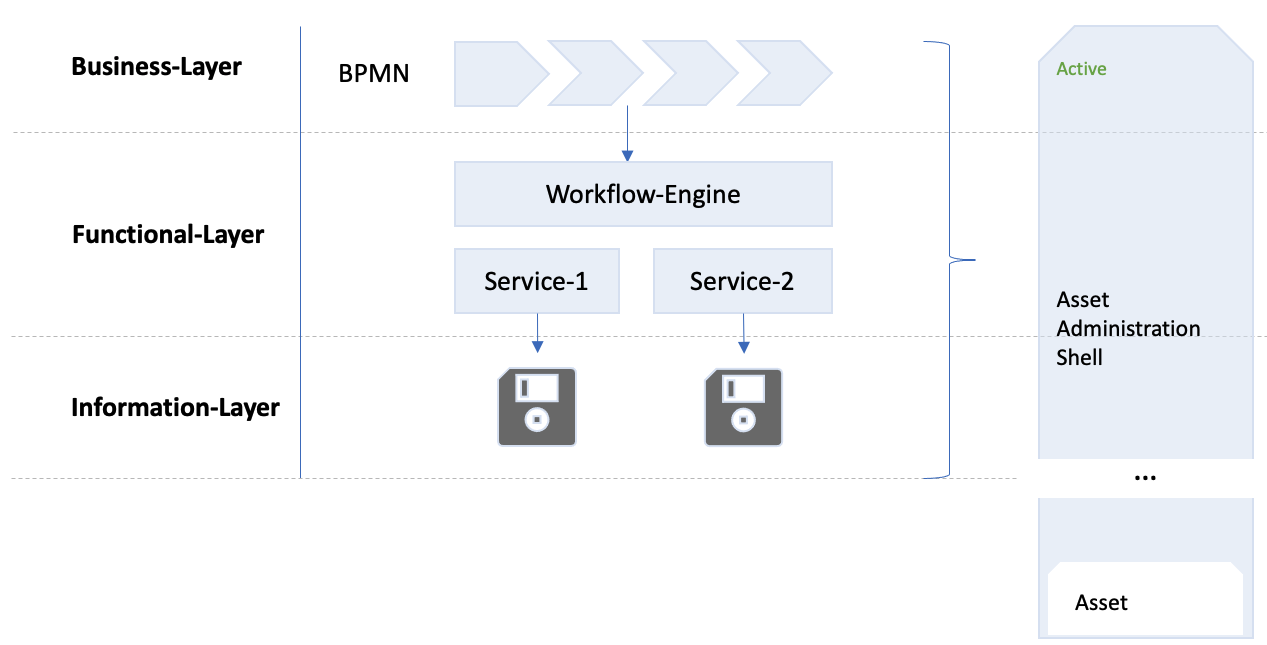
\includegraphics[scale=0.32]{content/pictures/tech_independent_architecture.png}
\caption{Technology independent architecture}
\source{Own illustration}
\label{fig:techn-indep-architecture}
\end{figure}

In the business layer, the processes representing the business models are described using \ac{BPMN}. Describing processes using \ac{BPMN} has two advantages: On the one hand, this representation creates transparency with regards to the services or activities to be executed, even for non-technical people. Likewise, non-technical people can create and manage the process mappings. On the other hand, processes can directly be executed with the help of workflow engines using \ac{BPMN}. For this purpose, the workflow engine is called with the defined process. The workflow engine then sequentially calls the activities defined in the process, by addressing the services in the functional layer. The integration of the process notation in the \ac{AAS} can be realized via submodels. Depending on the use case as well as the composition of the \ac{AAS}, the anchoring can take place in different submodels. Optimally, the anchoring of the process notation would take place in an aggregate \ac{AAS}, as described in \ref{sec:design}. In the use case of predictive maintenance, the \textit{maintenance} submodel defined by \citeauthor{Cavalieri2020AShell} could be extended by a property \textit{maintenance process}, which stores the necessary process steps to execute in the event of a technical intervention. 

The activities within a process reference the submodels defined in the \ac{AAS}. The implementation and provisioning of the submodels is realized in small independent services, that are located in the functional layer. Depending on the complexity or scope of a submodel, the service can provide both one or multiple functionalities. In the use case of \citeauthor{Cavalieri2020AShell}, two services in the functional layer would be created: A \textit{condition monitoring} and \textit{maintenance} service. These services then provide the functionalities such as \textit{set maintenance task} or \textit{get task information} via the defined interface of the \ac{AAS} \footnote{The technological implementation of the services can be done in different ways. A concrete method to instantiate services from submodels is described by \citet[p. 7]{BraunischDistributedEinleitung}. From a technical point of view, the assignment of activities to functionalities would then be done by adding URLs to the activities in \ac{BPMN}, which can then be called via HTTP by the workflow-engine.}. However, when implementing workflow engines, care must be taken not to create a too strong coupling between the functional layer services and the workflow engine. By doing so, it would be worth considering whether the workflow engine should be replaced by a message-oriented infrastructure using a message broker. The discussion whether to use a message-oriented infrastructure or workflow engines is out of scope of this thesis. The intention is to present a design pattern and not a complete architecture.

\section{Design} \label{sec:design}

The described architecture in \ref{sec:general-aspects} is of rather abstract nature, which does not directly indicate the necessary steps for implementation. In the following section, step-by-step instructions will be given on how to implement this. The architecture will be explained on the basis of the use case of predictive maintenance from \citeauthor{Cavalieri2020AShell}. While the paper from \citeauthor{Cavalieri2020AShell} only deals with creating the information model based on the \ac{AAS}, this approach extends their findings by describing a \ac{RAMI4.0} compliant architecture for the implementation of predictive maintenance which conforms to the one elaborated in \ref{sec:general-aspects}. The first step in the implementation is the definition of the composition. The composition determines how the individual assets are digitized. This step is of particular importance as it directly influences steps two and three. In a second step, it must be defined, how the connection between the physical and virtual environment can be established with the help of information technologies. To this end, a corresponding technology must be defined for each layer in \ac{RAMI4.0}. Afterwards, an information model must be derived for each asset in the system,  that describes the properties and functionalities of the asset. The information model is then manifested and transferred into the submodels of the \ac{AAS}. In a final step, the processes specified by the business model are modeled using \ac{BPM} and the individual activities of the process are linked to the respective submodel in the \ac{AAS}.

\textbf{Step 1: Composition definition}

When defining the composition, the use case to be realized and the assets to be digitized must first be considered. In case of an asset group, the individual components must be identified and considerations must be given to whether they require their own \ac{AAS} or not. In order to derive a decision, it must be evaluated whether the component should be active or passive in terms of their role in value networks and to what extent the functionalities of the asset should be represented independently in the overall system. As already outlined in \ref{sec:assetadministrationshell}, an asset in \ac{RAMI4.0} can be described by several \ac{AAS}. Likewise, an \ac{AAS} can contain further \ac{AAS}. This results in a multitude of combinations for digitizing assets. For example, the milling station in the present case can be implemented as one large \ac{AAS}, in which all sub-components, such as the robot's gripper arm, are included. It is also conceivable that one \ac{AAS} is created for each individual sub-component, which are then aggregated in the \ac{AAS} of the overall system. The difficulty in digitizing assets in \ac{RAMI4.0} using the \ac{AAS} is hence to find the right abstraction based on the scenario the asset is used. 

In the following, three possible forms of composing the milling station will be presented, based on which the advantages of each form will be discussed. Finally, a conclusion is drawn which composition is most suitable for predictive maintenance. Figure \ref{fig:aas-modeling-alternatives} graphically shows the three forms.

\begin{figure}[h]
\centering
\subfigure[]{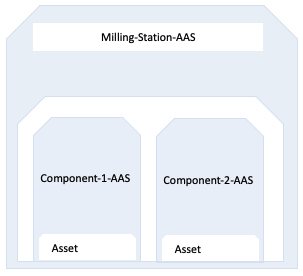
\includegraphics[width=.3\textwidth]{content/pictures/aas_version_1.png}}
\subfigure[]{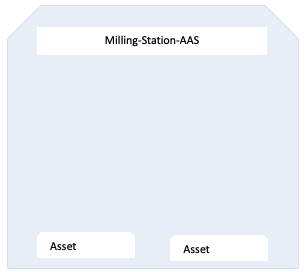
\includegraphics[width=.3\textwidth]{content/pictures/aas_version_2.png}}
\subfigure[]{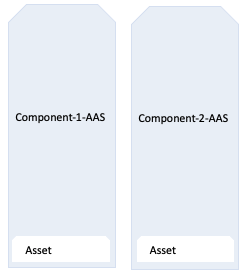
\includegraphics[width=.3\textwidth]{content/pictures/aas_version_3.png}}
\caption{Modelling alternatives for digitizing assets: (a) Asset Administration Shell from the individual components is aggregated on the root level, (b) all components are covered by a single Asset Administration Shell, (c) each component exposes its own Asset Administration Shell}
\source{Own illustration}
\label{fig:aas-modeling-alternatives}
\end{figure}

Figure \ref{fig:aas-modeling-alternatives} (a) shows that each component in the milling station is modeled with its own \ac{AAS}. The individual components are aggregated into one \ac{AAS} which is then exposed to the network. This type of composition has advantages in reducing complexity while modelling the individual submodels of the \ac{AAS}. This is especially the case if the components of the milling station are delivered by different manufacturers. To this end, each component manufacturer equips its component with an \ac{AAS}. The operator of the asset would then aggregate the individual \ac{AAS} into the milling station \ac{AAS}, which exposes the required properties and functionalities through one interface. In addition to the reduced complexity in modelling, this type of composition has advantages in \ac{SOA}. By addressing one component in the network, communication overhead and complexity can be reduced.

In Figure \ref{fig:aas-modeling-alternatives} (b) all properties and functionalities of an asset are modeled in one \ac{AAS}. For assets with many sub-components, this type of composition can quickly lead to high complexity in the submodels. However, this type of composition has the advantage, that hardware requirements can be reduced. This is especially the case for \ac{AAS}, that are active but do not have \ac{I4.0} communication capabilities. All functionalities and properties could be provided via one \ac{SBC} or \ac{OPCUA} server.

Figure \ref{fig:aas-modeling-alternatives} (c) shows the type of composition, which has the least coupling between the individual components. It is similar to the composition in \ref{fig:aas-modeling-alternatives} (a), without the aggregation in the milling station \ac{AAS}. For this purpose, each component of the milling station provides its functionalities and properties in the network itself. This type of composition has particular advantages when optimizations are to be realized with regard to latency or information access. For example, it is conceivable that the \ac{AAS} of component 1 is provided by the component itself using \ac{OPCUA} at the edge. The provisioning of component 2's \ac{AAS} can be realized in the cloud, since latencies in communication play a minor role. 

Variant (a) is particularly recommended for the implementation of predictive maintenance, as it offers the greatest flexibility in terms of provisioning and implementation of functionalities in cloud and edge and at the same time offers the possibility of aggregation reducing network overhead. The two options, cloud and edge, of provisioning an \ac{AAS} are especially important for use cases that work with real-time data.

\textbf{Step 2: IT-Platform}

After the type of digitization has been determined in step one, the connection between the physical and virtual world  must be established in a second step. For this purpose, the technical resources that meet the requirements for communication and processing of data must be selected. The requirements are derived directly from the selected composition. Figure \ref{fig:technology-map} provides an overview of possible technologies that are available for realizing different compositions. The outlined technologies are aligned with the layers of \ac{RAMI4.0}.

\begin{figure}[h]
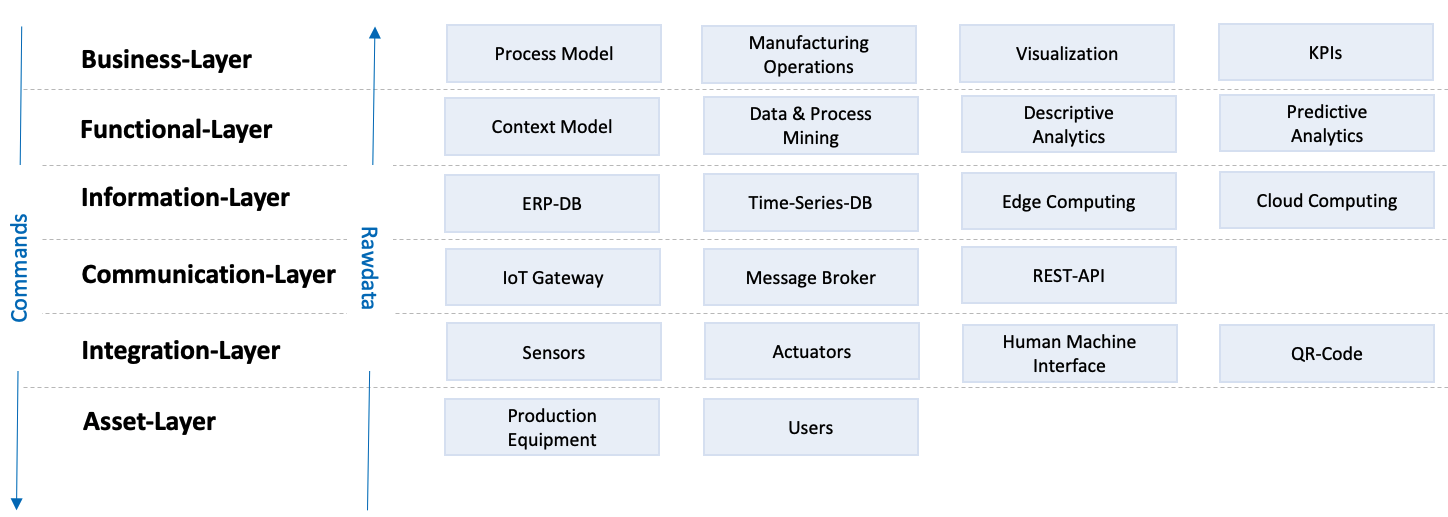
\includegraphics[scale=0.31]{content/pictures/rami_40_tech_mapping.png}
\caption{Technology map in the layers of RAMI4.0}
\source{Own illustration}
\label{fig:technology-map}
\end{figure}

In most cases, the asset is integrated into the virtual world using sensors or actuators in the integration layer. The generated data is then forwarded via an \ac{IIOT} gateway in the communication layer with \ac{I4.0} communication capabilities to the information layer, which stores and further processes the data in the \ac{AAS}. For the processing of time series and real-time data in the information layer, time series databases are the best choice, whereas relational databases are suitable for the storage of structural data. In the use case of predictive maintenance, a decision in favor of composition (a) from step one was made. Consequently, a separate \ac{AAS} is created for each component in the system, which is then combined in the system \ac{AAS}. This type of composition allows each component to use the optimal selection of technology to realize its functionality. This means that, for example, component 1 provides its data via an \ac{IIOT} gateway, while component 2 does so via a message broker using \ac{MQTT}. 

In order to derive a suitable selection of technologies, the requirements of the individual components must be defined in terms of networking, latency and required computing power. While a concrete decision regarding the requirements always depends on the specific environment, predictive maintenance is to be implemented, figure \ref{fig:technology-map-pred-maint} shows a selection of technologies that could be considered for implementing predictive maintenance. 

\begin{figure}[h]
\centering
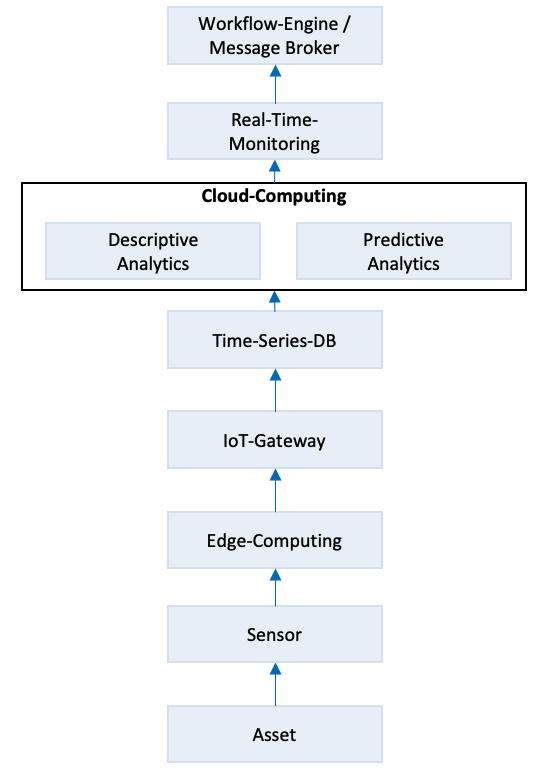
\includegraphics[width=.5\textwidth]{content/pictures/tech_map_pred_maintenance.png}
\caption{Technology map predictive maintenance}
\source{Own illustration}
\label{fig:technology-map-pred-maint}
\end{figure}

The two elements Cloud-Computing and Edge-Computing are particularly noteworthy. The provisioning of functionalities of the \ac{AAS} that require low latency can be realized at the edge. Functionalities that require intensive computing power but have lower latency requirements can be implemented in the cloud. The interoperable description of the functionalities in the submodels of the \ac{AAS} likewise allows the technologies to be exchanged seamlessly. Functionalities that are realized in the cloud can also be executed on the edge, given that the requirements regarding computing capacities are met.

\textbf{Step 3: Design of \ac{AAS}}

After defining the composition in step one and the technological infrastructure in step two, step three involves designing the information model for the individual elements of the composition. In doing so, the individual properties and functionalities of the asset must be transferred into submodels according to the property principle. For this purpose, it is suitable to divide the properties and functionalities of the asset into logical blocks. A logical block is a grouping that represents a specific aspect of the asset. If possible, standardized templates should be used to model interoperable properties and functions. For all properties that are not already provided in templates, standardized properties such as eclass should be used. \citet[p. 8, 10]{Cavalieri2020AShell} already provide a comprehensive information model, so that the modeling will not be shown in detail in this thesis.  However, a good possibility to get started with the design of an information model is provided by the package explorer through the Industry 4.0 platform \footnote{The package explorer is currently only available for the Windows platform and can be downloaded here: https://github.com/admin-shell-io/aasx-package-explorer}.

\textbf{Step 4: Design of business processes}

In the final step, the business model must be transformed into a process model with the help of \ac{BPMN}. To do this, the data needed to make decision within the process must be defined, as well as the activities that are to be performed. The activities of the process are linked to the services from the functional layer, in which the functionalities of the asset are mapped. It is recommended to define a process segment for each identified logical block from step three. Figure \ref{fig:pred-maintenance} shows an example process for predictive maintenance, which can be used to orchestrate the individual services in the functional layer.

\begin{figure}[h]
\centering
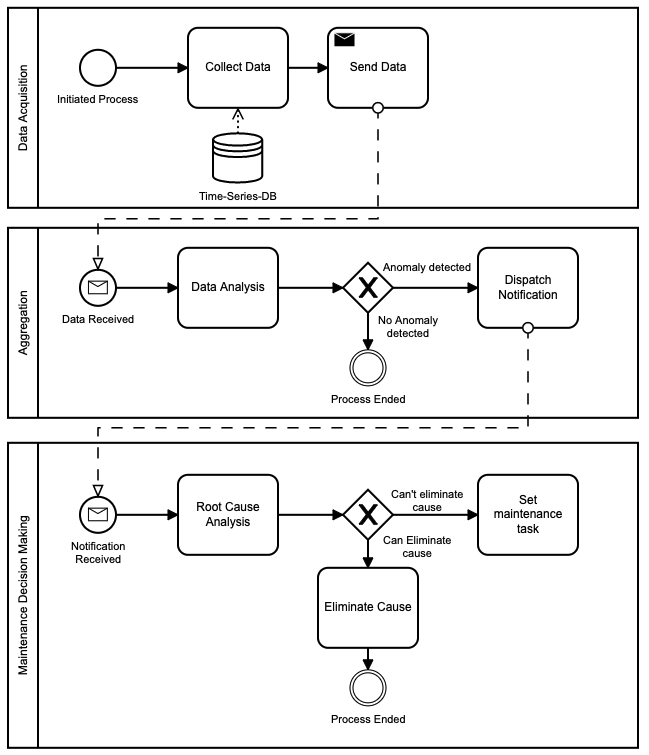
\includegraphics[width=.6\textwidth]{content/pictures/business_process_notation.png}
\caption{Business process for predictive maintenance}
\source{Own illustration}
\label{fig:pred-maintenance}
\end{figure}


\section{Roadmap to Industrial Digital Twin}
The instructions for implementing the \ac{AAS} and associated business processes shown in section \ref{sec:design} are applicable to an asset or asset group. In order to not limit the implementation to one asset or asset group, a roadmap is necessary that holistically enables the transformation of companies towards \ac{I4.0}. The introduction of \ac{RAMI4.0}, the \ac{AAS} and the accompanying transformation towards \ac{SOA} can present companies with a challenge. Companies will not be able to adopt directly the development of active \ac{AAS} and adapt their business processes accordingly as described in the previous chapter. Rather, a step-by-step transformation will be required to adapt an organization to the \ac{SOA} proposed by \ac{RAMI4.0} as well as the \ac{AAS}. To this end, the first step is to validate the already implemented measures and derive a development plan. A good framework for classifying and evaluating the current adoption of \ac{RAMI4.0} is provided by the maturity index, developed by \cite[p. 15]{Schuh2020IndustrieAcatech}. The maturity index consists of six successive steps through which adoption of \ac{I4.0} can be evaluated. These are \textit{Compute}, \textit{Connect}, \textit{Visible}, \textit{Transparent}, \textit{Predict} and \textit{Adapt}. \textit{Compute} describes the use of separate, unrelated information technologies, such as \ac{CNC}, to increase efficiency and reduce error rates \cite[p. 15]{Schuh2020IndustrieAcatech}. While \textit{Compute} introduces isolated information technologies, \textit{Connect} is concerned with the connection of individual production resources on the shop floor via \ac{API}s, which attempt to map the business processes. This can be done with the help of tools like \ac{MES} or \ac{ERP} \cite[p. 16]{Schuh2020IndustrieAcatech}. The two successive steps are referred to by the authors as the digitization, which lay the foundation for the implementation of \ac{I4.0} and the \ac{AAS}. The first step towards implementing \ac{I4.0} is \textit{Visible}. In this step, real-time capabilities are implemented for the assets on the shop floor. The real-time capabilities enable human decision making on based on the current status of the asset. \textit{Visible} also enables the connection of different data systems in the company such as \ac{MES} with \ac{ERP} \cite[p. 17]{Schuh2020IndustrieAcatech}. The available real-time-data is afterwards aggregated, analyzed and related data sets are linked to it. Therefore, this step is called \textit{Transparent}. The aim of this step is to use Big Data technologies to identify errors, monitor assets and establish impact correlations between the individual data sets. \textit{Predict} is defined as the ability to make predictions about future behaviour from historical and real-time data, so that potential problems can be identified in advance and appropriate action can be taken \cite[p. 19]{Schuh2020IndustrieAcatech}. If the actions to be taken are decided and executed by a system component itself without human interaction, one speaks of \textit{Adapt}, which represents the final step in the development of \ac{I4.0}. 

While the index represents a maturity model, \ac{RAMI4.0} provides a reference model with which companies can achieve the vision of \ac{I4.0}. However, \ac{RAMI4.0} only provides the organizational and technical parameters, but not a medium for evaluating the technical and organizational transformation. To assess the transformation of a company and thus the maturity level, the individual steps of the index are plotted on the Y-axis and the layers of \ac{RAMI4.0} on the X-axis. This makes it possible to derive a roadmap for the implementation of the individual layers of \ac{RAMI4.0} and to evaluate the opportunities it brings. Figure \ref{fig:roadmap} graphically establishes the relationship between the maturity model and \ac{RAMI4.0}.

\begin{figure}[h]
\centering
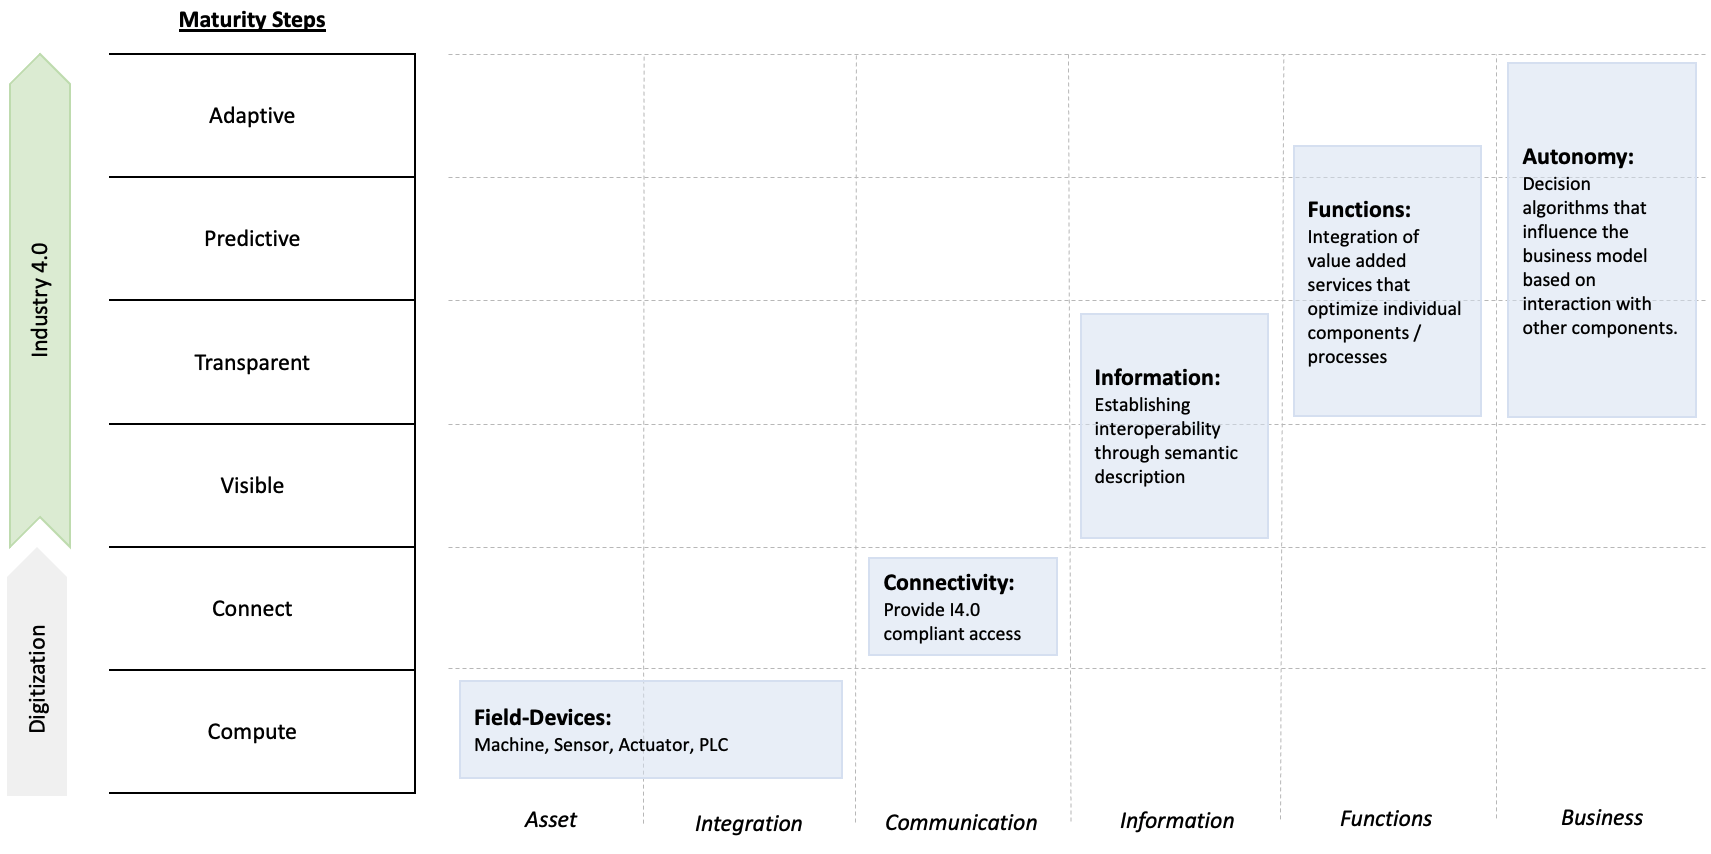
\includegraphics[scale=0.25]{content/pictures/rami_roadmap.png}
\caption{Roadmap for implementing RAMI4.0 based on the maturity index}
\source{Own illustration}
\label{fig:roadmap}
\end{figure}

The first two steps to enable the digitization of assets are computerization and connectivity. For this purpose, the assets must be equipped with sensors, actuators or PLCs in the asset layer of \ac{RAMI4.0}. In a second step, these must be connected with each other through \ac{I4.0} compatible technologies, such as \ac{IIOT} gateways. This includes, for example, retrofitting assets that do not currently have \ac{I4.0} communication capabilities, or replacing them with \ac{I4.0} compatible assets. Once the foundation for \ac{I4.0} has been laid through digitization, the assets can be described with the help of the \ac{AAS} in order to establish interoperability. The introduction of the \ac{AAS} will enable companies for the first time to view and store data from the shop floor in real-time. Given that the data is prepared graphically, for example in a dashboard, initial conclusion or measures can be derived based on the collected and stored data. While this data is primarily suitable for optimizing internal processes and reducing costs, the first added value for customers can be achieved by introducing predictive capacities in the functional layer. For this purpose, the previously purely passive \ac{AAS} must be converted into active \ac{AAS} and the functionalities must be mapped in the submodels. The functionalities of the submodels must then be provided in the form of services on the functional layer. By introducing \ac{BPM} and mapping business models in processes in the business layer, \textit{Adapt} can be realized. For this purpose, the processes are executed with the help of workflow engines, which call the services in the functional layer. This type of interaction then leas to decisions being made autonomously, with the aim of achieving end-to-end optimization of all processes in the company. 

An important insight that emerges from the roadmap is that the implementation of \ac{RAMI4.0} and the \ac{AAS} does not have to happen all at once. Rather, this can be done step by step. However, when implementing the individual steps, one should always be clear about the added value that can be realized as a result.